\section{Introducción}\label{intro}

\begin{frame}
    \begin{columns}[t]
        \begin{column}{.5\textwidth}
          \tableofcontents[sections={1-2},currentsection]
        \end{column}
        \begin{column}{.5\textwidth}
          \tableofcontents[sections={3-4},currentsection]
        \end{column}
    \end{columns}
\end{frame}

\subsection{¿Qué es Moogle!?}
\begin{frame}{¿Qué es Moogle!?}
\begin{center}
El proyecto “Moogle!” es una aplicación cuyo propósito es buscar inteligentemente un texto en un conjunto de documentos. 

\begin{figure}[h]
    \center
    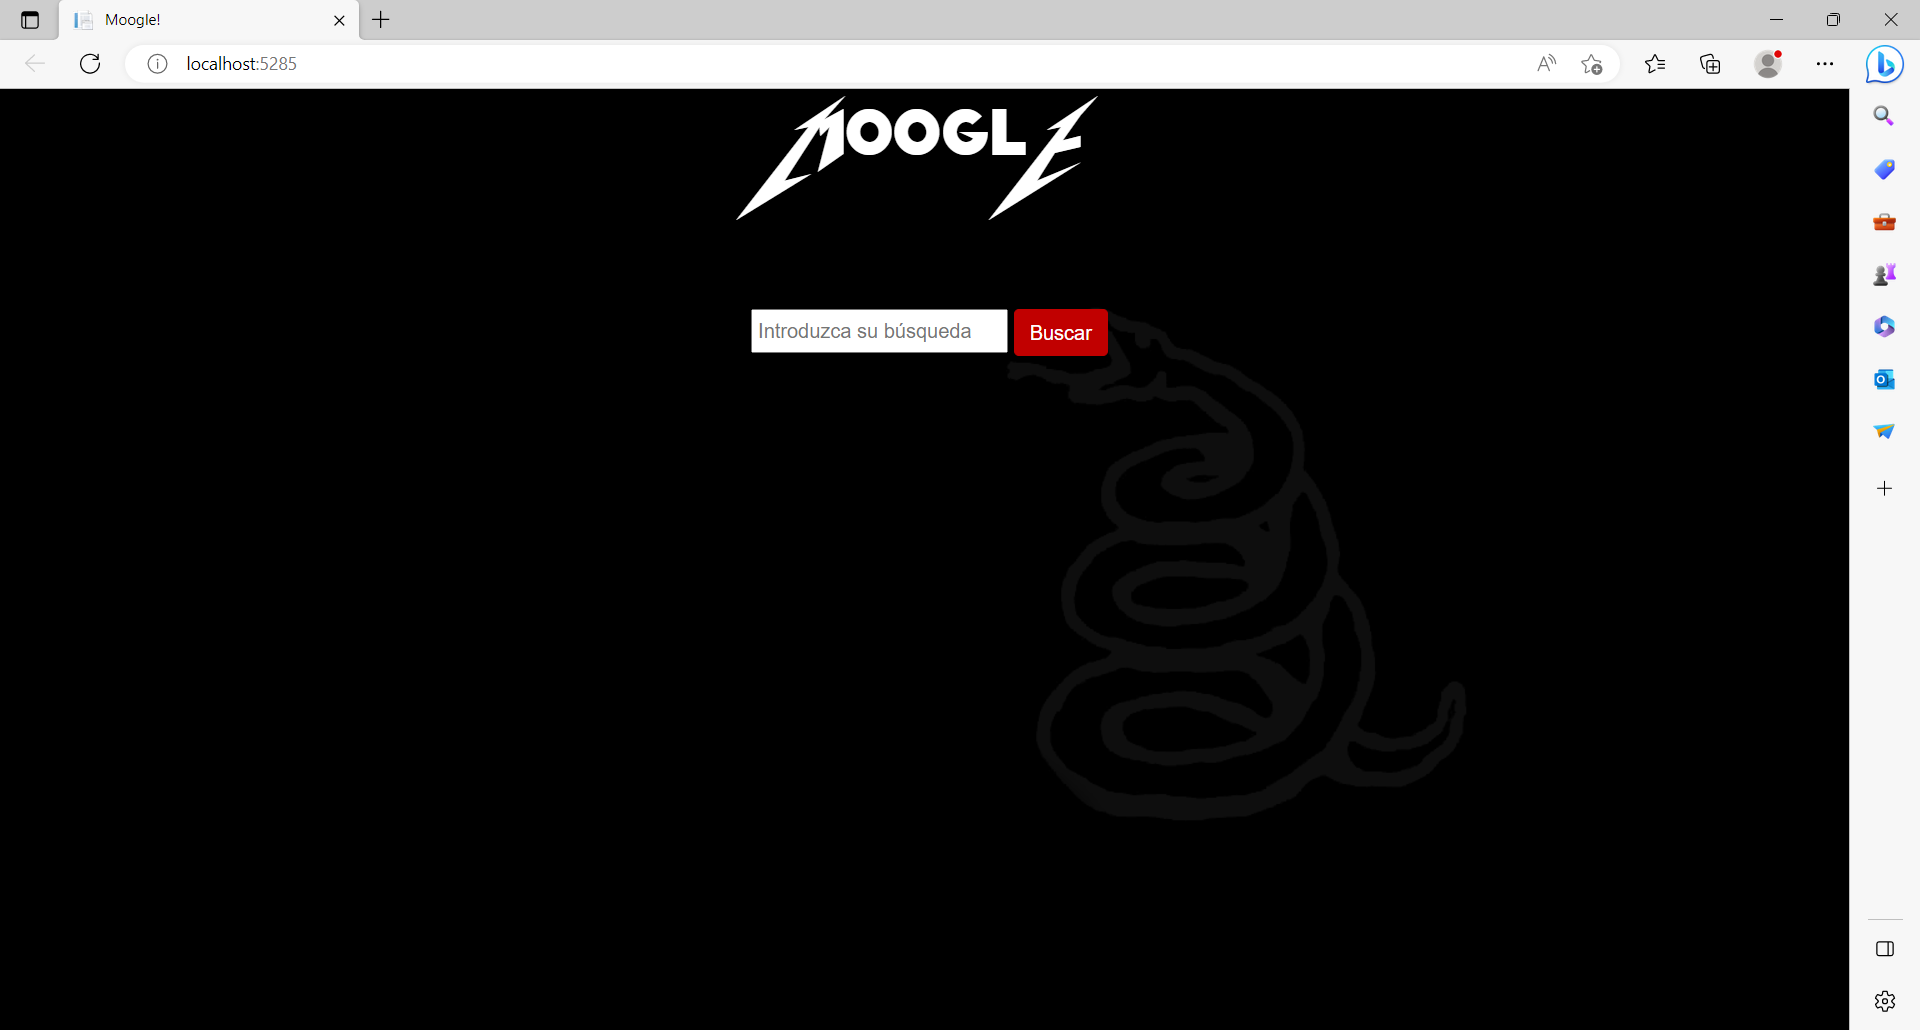
\includegraphics[width=5cm]{interfaz.png}
    \caption{Interfaz de Moogle!}
\end{figure}

\end{center}

\end{frame}


\subsection{Características}
\begin{frame}{Características}

Características:
\begin{itemize}
  \item Realiza búsquedas en un conjunto de documentos
  \item Devuelve resultados organizados por relevancia y de manera rápida
  \item Admite operadores de búsqueda básicos
  \item Muestra un snippet y realiza sugerencias
\end{itemize}

\end{frame}



